\documentclass{article}

\usepackage{arxiv}

\usepackage[utf8]{inputenc} % allow utf-8 input
\usepackage[T1]{fontenc}    % use 8-bit T1 fonts
\usepackage{hyperref}       % hyperlinks
\usepackage{url}            % simple URL typesetting
\usepackage{booktabs}       % professional-quality tables
\usepackage{amsfonts}       % blackboard math symbols
\usepackage{nicefrac}       % compact symbols for 1/2, etc.
\usepackage{microtype}      % microtypography
\usepackage{graphicx}
\usepackage{natbib}
\usepackage{doi}

\usepackage{amsmath}
\usepackage{nicematrix}
\usepackage{cleveref}
\usepackage{listings}
\usepackage{pgfplots}

\usepackage{algpseudocode}
\usepackage{algorithm}

\renewcommand{\algorithmicrequire}{\textbf{Input:}}
\renewcommand{\algorithmicensure}{\textbf{Initialize:}}

\NiceMatrixOptions{cell-space-top-limit=5pt,cell-space-bottom-limit=5pt,columns-width=20pt}

\crefname{lstlisting}{listing}{listings}
\Crefname{lstlisting}{Listing}{Listings}


% Listing options
\definecolor{codegreen}{rgb}{0,0.6,0}
\definecolor{codegray}{rgb}{0.5,0.5,0.5}
\definecolor{codepurple}{rgb}{0.58,0,0.82}
\definecolor{backcolour}{rgb}{0.95,0.95,0.92}

\lstdefinestyle{python_style}{
    backgroundcolor=\color{backcolour},
    commentstyle=\color{codegreen},
    keywordstyle=\color{magenta},
    numberstyle=\tiny\color{codegray},
    stringstyle=\color{codepurple},
    basicstyle=\ttfamily\footnotesize,
    breakatwhitespace=false,
    breaklines=true,
    captionpos=b,
    keepspaces=true,
    numbers=left,
    numbersep=5pt,
    showspaces=false,
    showstringspaces=false,
    showtabs=false,
    tabsize=2
}
\lstset{style=python_style}

\def\R{\mathbb{R}}


\title{EBREG-RL: Example-Based Regular Expression Generator
via Reinforcement Learning}

%\date{September 9, 1985}	% Here you can change the date presented in the paper title
\date{} 					% Or removing it

\author{
  \hspace{1mm}Dmitry Beresnev\\
	AIDS-MS1, Innopolis University\\
	\texttt{d.beresnev@innopolis.university}\\
	\And{}
  \hspace{1mm}Vsevolod Klyushev\\
	AIDS-MS1, Innopolis University\\
	\texttt{v.klyushev@innopolis.university}	\And{}
  \hspace{1mm}Nikita Yaneev\\
	AIDS-MS1, Innopolis University\\
	\texttt{n.yaneev@innopolis.university}
}

% \renewcommand{\undertitle}{\textbf{Group 1} Report for HDDA F24 course}
\renewcommand{\headeright}{}

\pgfplotsset{compat=1.18}
\begin{document}
\maketitle


\section{Introduction}

Nowadays big-tech companies increasingly prefer data-driven development, which requires careful extraction of 
information, including from unstructured or almost unstructured text. This task is considered as extremely tough, 
but in many real-world scenarios even unstructured text information have underlying syntactic pattern that can be 
characterized by a regular expressions, due to their adaptability and expressiveness.
However, even for experienced programmers, writing RegEx by hand is a boring, time-consuming, and error-prone 
process. Moreover, despite widespread use of regular expression, there are not so many researches and literature on 
the automatic RegEx generation. That is why we chose an example-based RegEx generation as a topic of the project of 
this course.

\begin{figure}[H]
  \centering
    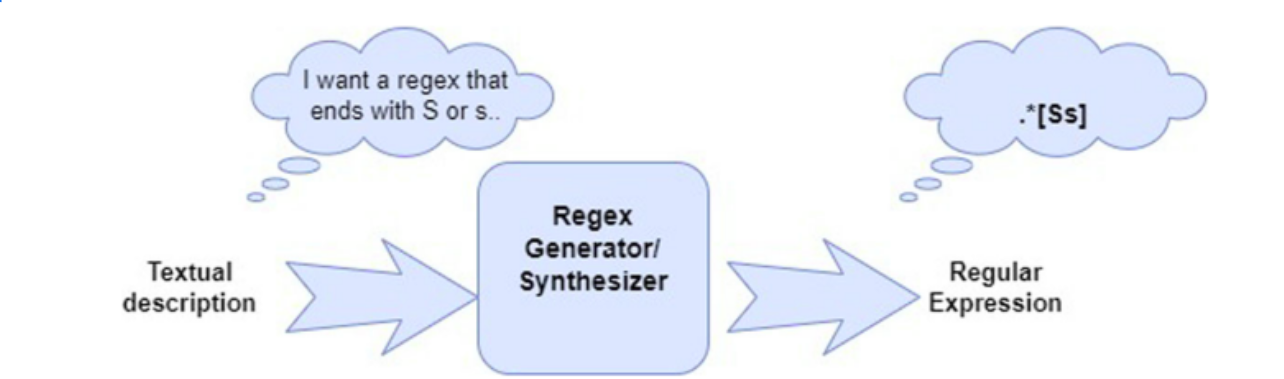
\includegraphics[width=0.5\textwidth]{./pictures/approach1.png}
    \caption[NL2RE pipeline]{NL2RE pipeline}\label{fig:NL2RE}
\end{figure}

One approach \cite{Zhong2018, Tariq2024} uses LLMs to convert natural language prompts into regular expressions (NL2RE). 
This method offers flexibility, allowing the model to generate a wide variety of RegExes. 
However, it requires significant computational resources and careful architecture design. 
This method is not ideal for generating RegExes that are specifically tailored to a particular domain or task. 
It is also challenging to ensure that the generated RegExes are accurate and efficient.

Another approach \cite{Bartoli2016, Bartoli2018} uses genetic programming (GP) to generate regular expression for specific tasks based on labeled 
data. The GP algorithm searches for the best-performing regular expression by iteratively evolving a population of 
candidate solutions. This method requires careful design of hyperparameters, such as the size of the population and 
the mutation rate, as well as a well-defined fitness function to evaluate the performance of each regular expression.

\section{Problem formulation}

We propose a new approach that leverages reinforcement learning (RL) to generate regular expression. 
This method formulates the regular expression generation process as a Markov decision process (MDP) 
with fully-observable deterministic episodic environment.

Each action corresponds to a regular expression syntax unit, state space would be a set of all possible sequences 
of syntax units of fixed length. For reward function various information retrieval metrics can be used as indicators 
of how good the generated regular expression is.

\subsection{Reverse Poland Notation}
Due to the fact that regular expressions have operations with different precedence and number of arguments, 
we decided to use the Reverse Polish Notation (RPN) for the construction of regular expressions.

In our RPN implementation we have 101 different actions:
\begin{itemize}
  \item 93 tokens (letters, difits, quantifiers, finish token, etc.),
  \item 2 binary operations ("concat" and "|"),
  \item 3 unary operations ("*", "+", "?"),
  \item 3 many to one operations ("[]", "\^[]", concat\_all").
\end{itemize}

\subsection{Action Space}
Action space for our RL agent consists of all possible actions for RPN.

\subsection{State Space}
The state space consists of $n$ placeholders, where each placeholder can either contain an action 
from the action space or remain empty (denoted by a special empty token).
To derive the current regular expression (state), we iterate over the non-empty tokens and apply the corresponding 
actions using Reverse Polish Notation (RPN).

\subsection{Dataset}
\dots

\subsection{Reward}
Reward function is a major part of RL pipeline. We come up with 2 approaches for reward calculation. 
Note, that we will calculate such rewards only by the end of the episode. Before that we will give 0 as reward.
Let's start with common parts.

First, we start with a text from which we want to extract specific information. To do this, we need to:
Identify the indices of the characters we want to retrieve.
Construct a "target bit mask" of length $n$ (where $n$ is the text length), where:
\begin{itemize}
  \item 1 marks positions to be included.
  \item 0 marks positions to be excluded.
\end{itemize}

Then, we get the current regular expression from RPN and apply it to the text, retriving indices of founnd symbold.
After that, we construct the "current bit mask" in the same way, as "target bit mask"

\subsubsection{Simple approach}
First idea of the reward is the following:
$$
\alpha \cdot \sum(A \oplus B) + \beta \cdot |C - D| + \gamma \cdot E
$$
where:
\begin{itemize}
  \item A - "target bitmask"
  \item B - "current bitmask"
  \item C - number of target words
  \item D - number of words, retrieved with regexp
  \item E - token length of regexp
\end{itemize}

\subsubsection{Complex approach}
Second idea of the reward is based on the fact, that we can calculate accuracy, precision, recall and F1 on bitmasks.
Thus reward function would be the following:
$$
\alpha \cdot F1 + \beta \cdot P + \gamma \cdot R + \delta \cdot |C - D| + \omega \cdot E\
$$
where:
\begin{itemize}
  \item F1 - F1 score on bit masks
  \item P - Precision on bit masks
  \item R - Recall on bit masks
  \item C - number of target words
  \item D - number of words, retrieved with regexp
  \item E - token length of regexp
\end{itemize}

\section{RL approaches}
We decided to check 2 RL approaches - Actor-Critic and Reinforce.

\subsection{Actor-Critic}
For Actor-Critic approach we define Neural Network (NN) with two heads: one for policy and one for state value.
The training procedure is the following:
\begin{algorithm}[H]

\caption{Actor-Critic}\label{algo:a2c}
\begin{algorithmic}[0]
  \Require{empty state of size $n$, environment $env$}

  \State{$done \gets False $}
  \State{$actions \gets [] $}
  \State{$states \gets [] $}
  \State{$rewards \gets [] $}
  \State{$state \gets env.reset() $}
  \While{$!done$}
  \State{$logits \gets net(state)[0]$}
  \State{$action \gets choose\_action(logits)$}
  \State{$new\_state, reward, done \gets env.step(action)$}
  \State{$actions, states, rewards \gets action, state, reward$}
  \EndWhile{}
  \State{$cumulative\_rewards \gets accomulate(rewards)$}
  \State{$logits, values \gets net(states)$}
  \State{$loss\_val \gets MSE(values, cumulative\_rewards)$}
  \State{$log\_probs \gets LogSoftmax(logits)$}
  \State{$adv \gets cumulative\_rewards - values$}
  \State{$log\_probs\_actions \gets adv \cdot log\_probs$}
  \State{$loss\_policy \gets -mean(log\_probs\_actions)$}
  \State{$probs \gets Softmax(logits)$}
  \State{$entropy \gets mean(sum((probs \cdot log\_probs),dim=1))$}
  \State{$entropy_loss \gets \beta \cdot entropy$}
  \State{$loss\_policy.backward()$}
  \State{$loss\_val \gets entropy_loss + loss\_val$}
  \State{$loss\_val.backward()$}
  
  \State{\Return{$net$}}

\end{algorithmic}
\end{algorithm}

\subsection{Reinforce}
\dots

\section{Experiments}
We decided to check our models on 3 different experiments:
\begin{itemize}
  \item Digits retrieval
  \item Retrieval of words, that consists of certain characters
  \item Email addressed retrieval
\end{itemize}

\section{Results and Discussion}
\dots

\section{Conclusion}
\dots

\begin{figure}[H]
  \centering
    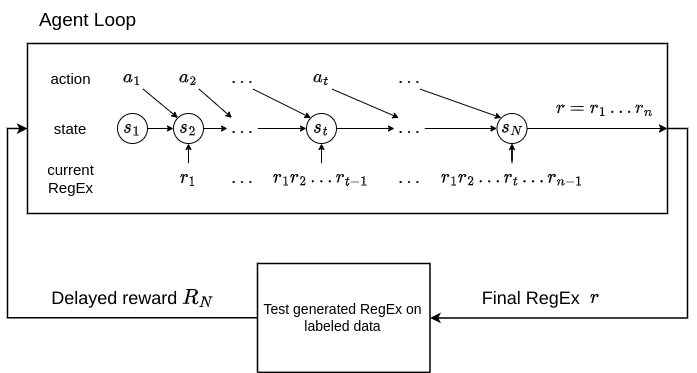
\includegraphics[width=0.5\textwidth]{./pictures/pipeline.png}
    \caption[our pipeline]{our pipeline}\label{fig:pipeline}
\end{figure}

\begin{figure}[H]
  \centering
    
\includegraphics[width=0.5\textwidth]{./pictures/rin.jpg}
    \caption[zhopa]{zhopa}\label{fig:zhopa}
\end{figure}


\section{Citation examples}
\cite{Zhong2018}~\cite{Bartoli2016}~\cite{Bartoli2018}~\cite{Tariq2024}


\bibliographystyle{plain}
\bibliography{references}



\end{document}

